%\documentclass[compress,t,11pt]{beamer}
\documentclass[handout,compress,t,11pt]{beamer}
\usetheme[]{metropolis}           % Use metropolis theme
\usefonttheme{serif}
\definecolor[named]{Gray}{RGB}{111,112,114}
\definecolor[named]{DarkGray}{RGB}{48,48,48}
\definecolor[named]{Cardinal}{RGB}{179,22,34}
\usepackage[T1]{fontenc}
\usepackage[altbullet]{lucidabr}
\usepackage{textcomp}
\usepackage{upquote} % needed to make straight quotes work in listings
\usepackage{listgolang}
\usepackage{mathtools}
\usepackage{comment}
\usepackage{tikz}
\usepackage{tikzsymbols}
 \usetikzlibrary{trees,shapes,plotmarks,arrows,er,automata,petri,topaths,positioning}
\usepackage{pifont}
\usepackage{clrscode}
\usepackage{setspace}
\usepackage{soul}
\usepackage{hyperref}
\usepackage{wasysym}

\setbeamercolor{palette primary}{fg=white,bg=Cardinal}
\setbeamercolor{palette secondary}{fg=white,bg=Gray}
\setbeamercolor{palette tertiary}{fg=white,bg=Cardinal}
\setbeamercolor{palette quaternary}{fg=white,bg=Gray}
\setbeamercolor{palette sidebar primary}{fg=white,bg=Cardinal}
\setbeamercolor{palette sidebar secondary}{fg=white,bg=Gray}
\setbeamercolor*{titlelike}{fg=Cardinal}
\setbeamercolor{structure}{fg=Gray}
\setbeamercolor{title separator}{fg=Cardinal}
\setbeamercolor{alerted text}{fg=Cardinal}
\setbeamercolor{reversed}{fg=Cardinal,bg=black}

\newcommand{\card}[1]{\ensuremath{\left|#1\right|}}
\newcommand{\norm}[1]{\ensuremath{\|#1\|}}

\title[Programming in Go]{\bf Programming in Go\\ Lesson 6: More Stuff}
\author{Matt Holiday} 
\institute[CP]{Cardinal Peak}
\date{21 May 2019} 
%\titlegraphic{\hfill
\includegraphics[width=.25\textwidth,height=.25\textheight]{cp-logo-2x.png}}
\titlegraphic{
\begin{tikzpicture}[overlay, remember picture,scale=0.4]
\node[at=(current page.north east), anchor=north east] (a) {};
\node[below left = 0.1cm and 0.1cm of a] (b)
{
\includegraphics[width=.25\textwidth,height=.25\textheight]{cp-logo-2x.png}};
\node[below left=2.2cm and 2.4cm of b]
{
\includegraphics[width=.2\textwidth]{gophercon-2019.png}};
\end{tikzpicture}}

\setbeamerfont{footline}{series=\bfseries\selectfont}
\setbeamersize{text margin left=12pt,text margin right=12pt}
\linespread{1.0}
\metroset{block=fill}

\hypersetup{
    colorlinks=true,
    linkcolor=Cardinal,
    filecolor=magenta,      
    urlcolor=blue,
}

\begin{document}
\frame{\titlepage} 

%\section{Introduction}
\begin{frame}[fragile]
    \frametitle{Lesson \#6}
    What we'll cover today:
    \begin{itemize}
    \item Homework \#5
    \item Enumerated types
    \item Variable argument lists
    \item Panic \& recover
    \item Reflection
    \item Custom JSON decoding via reflection
    \item Building for distribution
    \item Containerizing Go
    \item Discussion
    \end{itemize}
\end{frame}


% =================================================================================


\begin{frame}[fragile]
\frametitle{Homework \#5}
{\tiny
\begin{verbatim}
## who cares about the errors
## what matters is creating race conditions

$ go test -race .
got item=shoes&price=46 = 400 (<nil>)
got item=sandals&price=27 = 404 (<nil>)
got item=shoes = 400 (<nil>)
got item=socks&price=6 = 400 (<nil>)
got item=socks = 400 (<nil>)
got item=clogs&price=36 = 404 (<nil>)
got item=sandals = 400 (<nil>)
==================
WARNING: DATA RACE
Write at 0x00c000096d50 by goroutine 20:
got item=pants&price=30 = 404 (<nil>)
  runtime.mapassign_faststr()
      /usr/local/Cellar/go/1.11.5/libexec/src/runtime/map_faststr.go:190 +0x0
  hw5.database.add()
      /Users/mholiday/go/src/hw5/main.go:41 +0x295
  hw5.database.add-fm()
      /Users/mholiday/go/src/hw5/main.go:101 +0x65
  net/http.HandlerFunc.ServeHTTP()
      /usr/local/Cellar/go/1.11.5/libexec/src/net/http/server.go:1964 +0x51
  net/http.(*ServeMux).ServeHTTP()
      /usr/local/Cellar/go/1.11.5/libexec/src/net/http/server.go:2361 +0x191
  net/http.serverHandler.ServeHTTP()
      /usr/local/Cellar/go/1.11.5/libexec/src/net/http/server.go:2741 +0xc4
  net/http.(*conn).serve()
      /usr/local/Cellar/go/1.11.5/libexec/src/net/http/server.go:1847 +0x80a
\end{verbatim}}
\end{frame}

\begin{frame}[fragile]
\frametitle{Homework \#5}
{\tiny
\begin{verbatim}
Previous read at 0x00c000096d50 by goroutine 91:
  runtime.mapaccess2_faststr()
      /usr/local/Cellar/go/1.11.5/libexec/src/runtime/map_faststr.go:101 +0x0
  hw5.database.update()
      /Users/mholiday/go/src/hw5/main.go:51 +0x107
  hw5.database.update-fm()
      /Users/mholiday/go/src/hw5/main.go:102 +0x65
  net/http.HandlerFunc.ServeHTTP()
      /usr/local/Cellar/go/1.11.5/libexec/src/net/http/server.go:1964 +0x51
  net/http.(*ServeMux).ServeHTTP()
      /usr/local/Cellar/go/1.11.5/libexec/src/net/http/server.go:2361 +0x191
  net/http.serverHandler.ServeHTTP()
      /usr/local/Cellar/go/1.11.5/libexec/src/net/http/server.go:2741 +0xc4
  net/http.(*conn).serve()
      /usr/local/Cellar/go/1.11.5/libexec/src/net/http/server.go:1847 +0x80a

Goroutine 20 (running) created at:
  net/http.(*Server).Serve()
      /usr/local/Cellar/go/1.11.5/libexec/src/net/http/server.go:2851 +0x4c5
  net/http.(*Server).ListenAndServe()
      /usr/local/Cellar/go/1.11.5/libexec/src/net/http/server.go:2764 +0xe8
  net/http.ListenAndServe()
      /usr/local/Cellar/go/1.11.5/libexec/src/net/http/server.go:3004 +0xef
  hw5.runServer()
      /Users/mholiday/go/src/hw5/main.go:106 +0x376

. . .

==================
\end{verbatim}}
\end{frame}

\begin{frame}[fragile]
    \frametitle{Homework \#5}
    Test program:
\begin{golang}
package main // main_test.go

import (
	"fmt"
	"net/http"
	"os"
	"testing"
	"time"
)

type sku struct {
	item  string
	price string
}
\end{golang}
\end{frame}

\begin{frame}[fragile]
    \frametitle{Homework \#5}
\begin{golang}
var items = []sku{
	{"shoes", "46"},
	{"socks", "6"},
	{"sandals", "27"},
	{"clogs", "36"},
	{"pants", "30"},
	{"shorts", "20"},
}

func doQuery(cmd, parms string) {
	resp, err := http.Get("http://localhost:8000/" +
                          cmd + "?" + parms)
	if err == nil {
		defer resp.Body.Close()
	}
	fmt.Fprintf(os.Stderr, "got %s = %d (%v)\n", parms,
                resp.StatusCode, err)
}
\end{golang}
\end{frame}

\begin{frame}[fragile]
    \frametitle{Homework \#5}
\begin{golang}
func runAdds() {
	for {
		for _, s := range items {
			doQuery("create", 
                    "item="+s.item+"&price="+s.price)
		}
	}
}

func runUpdates() {
	for {
		for _, s := range items {
			doQuery("update", 
                    "item="+s.item+"&price="+s.price)
		}
	}
}
\end{golang}
\end{frame}

\begin{frame}[fragile]
    \frametitle{Homework \#5}
\begin{golang}
func runDrops() {
	for {
		for _, s := range items {
			doQuery("delete", "item="+s.item)
		}
	}
}

func TestServer(t *testing.T) {
	go runServer()

	go runAdds()
	go runDrops()
	go runUpdates()

	time.Sleep(30 * time.Second)
	t.Errorf("NO RACE?")
}
\end{golang}
\end{frame}

\begin{frame}[fragile]
    \frametitle{Homework \#5}
    New main program:
\begin{golang}
package main // main.go

import (
	"fmt"
	"log"
	"net/http"
	"strconv"
	"sync"
)

// NOTE: don't do this in real life
type dollars float32

func (d dollars) String() string {
	return fmt.Sprintf("$%.2f", d)
}
\end{golang}
\end{frame}

\begin{frame}[fragile]
    \frametitle{Homework \#5}
\begin{golang}
// We embed a sync.Mutex into the database but now it
// must be a struct and be passed by reference (ptr);
// it's not safe to copy a mutex

type database struct {
	sync.Mutex
	data map[string]dollars
}

func (db *database) list(w http.ResponseWriter, 
                         req *http.Request) {
	db.Lock()
	defer db.Unlock()

	for item, price := range db.data {
		fmt.Fprintf(w, "%s: %s\n", item, price)
	}
}
\end{golang}
\end{frame}

\begin{frame}[fragile]
    \frametitle{Homework \#5}
\begin{golang}
func (db *database) add(w http.ResponseWriter,
                        req *http.Request) {
	item := req.URL.Query().Get("item")
	price := req.URL.Query().Get("price")

	db.Lock()
	defer db.Unlock()

	if _, ok := db.data[item]; ok {
		w.WriteHeader(http.StatusBadRequest) // 404

		fmt.Fprintf(w, "duplicate item: %q\n", item)
		return
	}
\end{golang}
\end{frame}

\begin{frame}[fragile]
    \frametitle{Homework \#5}
\begin{golang}
	if f64, err := strconv.ParseFloat(price, 32); err != nil {
		w.WriteHeader(http.StatusBadRequest) // 400

		fmt.Fprintf(w, "invalid price: %q\n", price)
	} else {
		db.data[item] = dollars(f64)

		fmt.Fprintf(w, "added %s with price %s\n", item, 
                    dollars(f64))
	}
}
\end{golang}
\end{frame}

\begin{frame}[fragile]
    \frametitle{Homework \#5}
\begin{golang}
func (db *database) update(w http.ResponseWriter, 
                           req *http.Request) {
	item := req.URL.Query().Get("item")
	price := req.URL.Query().Get("price")

	db.Lock()
	defer db.Unlock()

	if _, ok := db.data[item]; !ok {
		w.WriteHeader(http.StatusNotFound) // 404

		fmt.Fprintf(w, "no such item: %q\n", item)
		return
	}
\end{golang}
\end{frame}

\begin{frame}[fragile]
    \frametitle{Homework \#5}
\begin{golang}
	if f64, err := strconv.ParseFloat(price, 32); err != nil {
		w.WriteHeader(http.StatusBadRequest) // 400

		fmt.Fprintf(w, "invalid price: %q\n", price)
	} else {
		db.data[item] = dollars(f64)

		fmt.Fprintf(w, "new price %s for %s\n", dollars(f64), 
                    item)
	}
}
\end{golang}
\end{frame}

\begin{frame}[fragile]
    \frametitle{Homework \#5}
\begin{golang}
func (db *database) fetch(w http.ResponseWriter, 
                          req *http.Request) {
	item := req.URL.Query().Get("item")

	db.Lock()
	defer db.Unlock()

	if _, ok := db.data[item]; !ok {
		w.WriteHeader(http.StatusNotFound) // 404

		fmt.Fprintf(w, "no such item: %q\n", item)
		return
	}

	fmt.Fprintf(w, "item %s has price %s\n", item, 
                db.data[item])
}
\end{golang}
\end{frame}

\begin{frame}[fragile]
    \frametitle{Homework \#5}
\begin{golang}
func (db *database) drop(w http.ResponseWriter, 
                         req *http.Request) {
	item := req.URL.Query().Get("item")

	db.Lock()
	defer db.Unlock()

	if _, ok := db.data[item]; !ok {
		w.WriteHeader(http.StatusNotFound) // 404

		fmt.Fprintf(w, "no such item: %q\n", item)
		return
	}

	delete(db.data, item)
	fmt.Fprintf(w, "dropped %s\n", item)
}
\end{golang}
\end{frame}

\begin{frame}[fragile]
    \frametitle{Homework \#5}
\begin{golang}
var db = database{data: map[string]dollars{"shoes": 50,
                                           "socks": 5}}

func runServer() {
	http.HandleFunc("/list", db.list)
	http.HandleFunc("/create", db.add)
	http.HandleFunc("/update", db.update)
	http.HandleFunc("/delete", db.drop)
	http.HandleFunc("/read", db.fetch)

	log.Fatal(http.ListenAndServe("localhost:8000", nil))
}

func main() {
	runServer()
}
\end{golang}
\end{frame}

% =================================================================================

\section{Odds and Ends}
\begin{frame}[fragile]
    \frametitle{Enumerated types}
    There are no real enumerated types in Go \par
    \vspace{0.5\baselineskip}
    You can make an almost-enum type using a named type and constants:
\begin{golang}
    type shoe int

    const (
        tennis shoe = iota
        dress
        sandal
        clog
    )
\end{golang}
    \vspace{0.5\baselineskip}
    \verb|iota| starts at 0 in each \verb|const| group and increments once \\
    on each successive line; here 0, 1, 2, ...
\end{frame}

\begin{frame}[fragile]
    \frametitle{Enumerated types}
    Traditional flags are easy: \par
\begin{golang}
type Flags uint

const (
    FlagUp Flags = 1 << iota // is up
    FlagBroadcast            // supports broadcast access
    FlagLoopback             // is a loopback interface
    FlagPointToPoint         // is a point-to-point link
    FlagMulticast            // supports multicast access
)
\end{golang}
 \vspace{0.4\baselineskip}
These flags take on the values in a power-of-two sequence:
 \verb|0x01|, \verb|0x02|, \verb|0x04|, etc. \par
 \vspace{0.6\baselineskip}
That makes them easy to combine, e.g. \verb@FlagUp | FlagLoopback@ 
\end{frame}

\begin{frame}[fragile]
    \frametitle{Enumerated types}
    Go also supports more complex \verb|iota| expressions: \par
\begin{golang}
type ByteSize int64

const (
	_            = iota // ignore first value
	KiB ByteSize = 1 << (10 * iota)
	MiB
	GiB
	TiB
	PiB
	EiB
)
\end{golang}
\vspace{2\baselineskip}
So \verb|EiB| is set to $2^{60} = 1152921504606846976 \approx 10^{19}$
\end{frame}

\begin{frame}[fragile]
    \frametitle{Iteration}
The \href{https://godoc.org/github.com/bradfitz/iter}{iter} package doesn't
allocate because \verb|struct{}| requires no space (originally released as an 
``educational joke'')
\vspace{0.4\baselineskip}
\begin{golang}
package main

import (
	"fmt"
	"github.com/bradfitz/iter"
)

func main() {
	for i := range iter.N(5) {
		fmt.Println(i)
	}
}
\end{golang}
\vspace{0.4\baselineskip}
The playground now has \href{https://play.golang.org/p/eqEo7mqdS9l}{3rd-party package} and
\href{https://play.golang.org/p/KLZR7NlVZNX}{multi-file} support!
\end{frame}

\begin{frame}[fragile]
    \frametitle{Variable argument lists}
    What if we don't know how many parameters a function needs?
\vspace{\baselineskip}
\begin{golang}
    fmt.Printf("%#v\n", myMap)
    
    fmt.Printf("%s: %s\n", type, quantity)
    
    a := sum(1, 2, 3)

    b := sum(1, 2, 3, 4, 5)
\end{golang}
\vspace{2\baselineskip}
All the formatted printing code uses variable argument lists
\end{frame}

\begin{frame}[fragile]
    \frametitle{Variable argument lists}
    We use a special operator \verb|...| before the parameter type
\begin{golang}
func sum(nums ...int) int {
    total := 0

    for _, num := range nums {
        total += num
    }

	fmt.Printf("+/%v=%d\n", nums, total)
    return total
}

// prints +/[1 2 3 4 5] = 15
\end{golang}
\vspace{\baselineskip}
Only the {\bf last} parameter may have this operator
\end{frame}

\begin{frame}[fragile]
    \frametitle{Variable argument lists}
    Since the parameter looks like a slice, we can pass a slice
\begin{golang}
func main() {
	fmt.Println(add())
	fmt.Println(add(11))
	fmt.Println(add(1, 2, 3, 4))

    s := []int{1, 2, 3}

    fmt.Println(add(s...))
}

// prints 0, 11, 10, 6
\end{golang}
\vspace{\baselineskip}
The special operator \verb|...| {\em after} the actual parameter
``unpacks'' it into the variable argument list
\end{frame}

% =================================================================================

\section{Error Handling}
\begin{frame}[fragile]
    \frametitle{Errors in Go}
When it comes to errors, you may fall into one of these camps:
\begin{enumerate}
\item you hate constantly writing if/else blocks
\vspace{0.4\baselineskip}
\item you think writing if/else blocks makes things clearer
\vspace{0.4\baselineskip}
\item {\bf you don't care because you're too busy writing code}
\end{enumerate}
\vspace{\baselineskip}
\begin{center}
 
\includegraphics[width=0.45\textwidth]{go-error-key.jpg}
\end{center}
\end{frame}

\begin{frame}[fragile]
    \frametitle{The two ways of handling errors}
    There are two main categories of errors:
    \begin{itemize}
        \item errors resulting from user input or environmental conditions; \\
        for example, a ``file not found'' error
        \vspace{0.4\baselineskip}
        \item errors resulting from invalid program logic; \\
        for example, a nil pointer
    \end{itemize}
    \vspace{2\baselineskip}
    Go handles the first case by returning the \verb|error| type \par
    \vspace{\baselineskip}
    For program logic errors, Go does a \verb|panic| \par
    \vspace{\baselineskip}
    Generally this will cause the program to crash with a traceback
\end{frame}

\begin{frame}[fragile]
    \frametitle{When your program has a logic bug}
\begin{center}
\vspace{0.4\baselineskip}

\includegraphics[width=0.95\textwidth]{fail-hard-fast.jpg} \par
\vspace{0.2\baselineskip}
{\bf Fail hard, fail fast}
\end{center}
\end{frame}

\begin{frame}[fragile]
    \frametitle{When should we panic?}
    Only when the error was caused by our own programming defect
    \begin{itemize}
        \item if we encoded something, then it should decode again
        \vspace{0.4\baselineskip}
        \item if we built a data structure, we should be able to walk it
        \vspace{0.4\baselineskip}
        \item we should recognize any message we send to ourselves
    \end{itemize}
    \vspace{\baselineskip}
    In other words, {\em \verb|panic| should be used when our assumptions of\\
    our own programming design or logic are wrong} \par
    \vspace{\baselineskip}
    These cases might use an ``assert'' in other programming languages \par
    % \vspace{\baselineskip}
    % We should not pass \verb|panic| to or through third-party code; use
    % \verb|recover| and pass an \verb|error| as usual
\end{frame}

\begin{frame}[fragile]
    \frametitle{When should we panic?}
    A \href{https://www.cs.cornell.edu/courses/cs3110/2009sp/recitations/rec25.html}%
       {\em B-tree} data structure satisfies several invariants:
    \begin{enumerate}
    \item every path from the root to a leaf has the same length
    \vspace{0.3\baselineskip}
    \item if a node has $n$ children, it contains $n-1$ keys
    \vspace{0.3\baselineskip}
    \item every node (except the root) is at least half full
    \vspace{0.3\baselineskip}
    \item the root has at least two children if it is not a leaf
    \vspace{0.3\baselineskip}
    \item subnode keys fall between the keys of the parent node
          that lie on either side of the subnode pointer
    \end{enumerate}
    \vspace{\baselineskip}
    If any of these is ever false, the B-tree methods should {\bf panic!}
    \vspace{0.4\baselineskip}
\begin{golang}
if node != root && !leaf(node) && len(node.children) < 2 {
    panic("internal node has too few children")
}
\end{golang}
\end{frame}

\begin{frame}[fragile]
    \frametitle{Exception handling}
    Exception handling was popularized to allow ``graceful degradation'' of
    safety-critical systems (e.g., Ada and flight control software)\par
    \vspace{2\baselineskip}
    Exception handling introduces many additional paths of execution
    that are effectively invisible in the code \par
    \vspace{2\baselineskip}
    Code with exceptions is harder to analyze \par
    \vspace{2\baselineskip}
    Ironically, most safety-critical systems are built without
    using exceptions!
\end{frame}

\begin{frame}[fragile]
    \frametitle{Exception handling}
    Officially, Go doesn't support exception handling as in other languages \par
    \vspace{\baselineskip}
    Practically, it does --- in the form of \verb|panic| \& \verb|recover| \par
    \vspace{\baselineskip}
    \verb|panic| in a function will still cause deferred function calls to run \par
    \vspace{\baselineskip}
    Then it will stop only if it finds a valid \verb|recover| call in a \verb|defer|\\
    as it unwinds the stack \par
\end{frame}

\begin{frame}[fragile]
    \frametitle{Panic and recover}
    Recovery from \verb|panic| only works inside \verb|defer|
\begin{golang}
func abc() {
    panic("omg")
}

func main() {
    defer func() {
        if p := recover(); p != nil {
            // what can you do?
            fmt.Println("recover:", p)
        }
    }()

    abc()
}

// prints recover: omg
\end{golang}
\end{frame}

\begin{frame}[fragile]
    \frametitle{Define errors out of existence}
    Error cases are one of the primary sources of complexity \par
    \vspace{0.4\baselineskip}
    The best way to deal with many errors is to make them impossible \par
    \vspace{0.4\baselineskip}
    Design abstractions so that all inputs are meaningful:
    \begin{itemize}
        \item deleting a non-existant item from a map
        \item taking the length of a nil slice (returns 0)
        \item reading from a nil map (returns a default value)
    \end{itemize}
    \vspace{\baselineskip}
    All these things reduce ``special-case'' logic that's hard to test and debug
    (or even think about!) \par
\end{frame}

% - which is why (ironically) that something introduced for safety gets
%   avoided in safety-critical code
% - the "safe" version of Ada (SPARK) removes, among other things:
%   * exceptions
%   * side effects in expressions
% - go reduces the use of both

\begin{frame}[fragile]
    \frametitle{Getting the bugs out}
    \begin{center}
    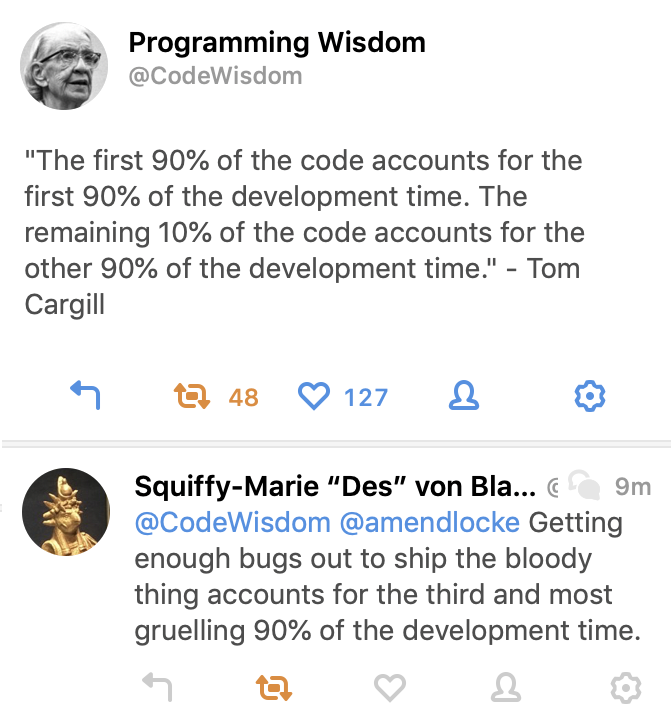
\includegraphics[height=.85\textheight]{bugs-out.png}
    \end{center}
\end{frame}


% =================================================================================

\section{Using Reflection}

\begin{frame}[fragile]
    \frametitle{Switching on type}
    \verb|interface{}| can be anything, since it has no methods \par
    \vspace{0.6\baselineskip}
    Which means it's a ``generic'' thing; we need its concrete type
    \vspace{0.6\baselineskip}
\begin{golang}
func Println(args ...interface{}) {
    buf := make([]byte, 0, 80)

    for arg := range args {
        switch a := arg.(type) {
            case string:
                buf = append(buf, a...)
            case fmt.Stringer:
                buf = append(buf, a.String()...)
            . . .
        }
    }
}
\end{golang}
\end{frame}

\begin{frame}[fragile]
    \frametitle{Type extraction}
    We can also extract a concrete type with a conversion \par
    \vspace{0.6\baselineskip}
    If we use the two-result version, we can avoid \verb|panic|
\begin{golang}
    data map[string]interface{}

    // this code panics if the conversion can't be made

	score := data["score"].(float64)

    // this code handles failure gracefully ...

	if intent, ok := data["intent"].(string); ok {
		w.Intent = intent
	} else {
		return fmt.Errorf("missing intent")
	}
\end{golang}
\end{frame}

\begin{frame}[fragile]
    \frametitle{Hard JSON}
    Not all JSON messages are well-behaved \par
    \vspace{0.4\baselineskip}
    What if some keys depend on others in the message?
{\small
\begin{verbatim}
{
  "item": "album", 
  "album": {"title": "Dark Side of the Moon"}
}

{
  "item": "song", 
  "song": {"title": "Bella Donna", 
           "artist": "Stevie Nicks"}
}
\end{verbatim}}
\vspace{\baselineskip}
You can't describe this easily using a fixed \verb|struct| definition
\end{frame}

\begin{frame}[fragile]
    \frametitle{Custom JSON decoding}
    We'll make a wrapper and a custom decoder \par
\begin{golang}
type response struct {
    Item   string `json:"item"`
    Album  string
    Title  string
    Artist string
}

type respWrapper struct {
    response
}
\end{golang}
\vspace{2\baselineskip}
We need the \verb|respWrapper| because it must have a separate
unmarshal function from the \verb|response| type (see below)
\end{frame}

\begin{frame}[fragile]
    \frametitle{Custom JSON decoding}
\begin{golang}
func (r *respWrapper) UnmarshalJSON(b []byte) (err error) {
    var raw map[string]interface{}

    // ignore error handling
    err = json.Unmarshal(b, &r.response)
    err = json.Unmarshal(b, &raw)

    switch r.Item {
    case "album":
        inner, ok := raw["album"].(map[string]interface{})
        
        if ok {
            if album, ok := inner["title"].(string); ok {
                r.Album = album
            }
        }
\end{golang}
\end{frame}

\begin{frame}[fragile]
    \frametitle{Custom JSON decoding}
\begin{golang}
    case "song":
        inner, ok := raw["song"].(map[string]interface{})

        if ok {
            if title, ok := inner["title"].(string); ok {
                r.Title = title
            }

            if artist, ok := inner["artist"].(string); ok {
                r.Artist = artist
            }
        }
    }

    return err
}
\end{golang}
\end{frame}

\begin{frame}[fragile]
    \frametitle{Custom JSON decoding}
\begin{golang}
func main() {
    var resp1, resp2 respWrapper
    var err error

    if err = json.Unmarshal([]byte(j1), &resp1); err != nil {
        log.Fatal(err)
    }

    fmt.Printf("%#v\n", resp1.response)

    if err = json.Unmarshal([]byte(j2), &resp2); err != nil {
        log.Fatal(err)
    }

    fmt.Printf("%#v\n", resp2.response)
}
\end{golang}
\end{frame}

\begin{frame}[fragile]
    \frametitle{Custom JSON decoding}
\begin{golang}
var j1 = `{
  "item": "album",
  "album": {"title": "Dark Side of the Moon"}
}`

var j2 = `{
  "item": "song",
  "song": {"title": "Bella Donna", "artist": "Stevie Nicks"}
}`



// main.response{Item:"album", Album:"Dark Side of the Moon",
//               Title:"", Artist:""}
//
// main.response{Item:"song", Album:"", Title:"Bella Donna",
//               Artist:"Stevie Nicks"}
\end{golang}
\end{frame}


\begin{frame}[fragile]
    \frametitle{Testing JSON}
    We want to know if a known fragment of JSON is contained
    in a larger unknown piece \par
{\small
\begin{verbatim}
{"id": "Z"} in? {"id": "Z", "part": "fizgig", "qty": 2}
\end{verbatim}}
    All done with reflection from a generic map
    \vspace{\baselineskip}
\begin{golang}
func contains(unknown, known map[string]interface{}) error {
	for k, v := range known {
	    switch x := v.(type) {
	    case string:
			if !matchString(k, x, unknown) {
				return fmt.Errorf("%s unmatched (%s)", k, x)
			}

        . . .
\end{golang}
\end{frame}

\begin{frame}[fragile]
    \frametitle{Testing JSON}
\begin{golang}
        . . .

		case map[string]interface{}:
			if v, ok := unknown[k]; !ok {
				return fmt.Errorf("%s missing", k)
			} else if u, ok := v.(map[string]interface{}); ok {
				if err := contains(u, x); err != nil {
					return fmt.Errorf("%s != %+v: %s", 
                                      k, x, err)
				}
			} else {
				return fmt.Errorf("%s not obj (%#v)", k, v)
			}
		}
	}

	return nil
}
\end{golang}
\end{frame}

\begin{frame}[fragile]
    \frametitle{Testing JSON}
\begin{golang}
func matchString(key, exp string, 
                 resp map[string]interface{}) bool {

    // if the key is present, extract the "any" value
    // and convert it to a string and test for equality

	if v, ok := resp[key]; ok {
		if val, ok := v.(string); ok && val == exp) {
			return true
		}
	}

	return false
}
\end{golang}
\end{frame}


% =================================================================================

\section{Building for Distribution}
\begin{frame}[fragile]
    \frametitle{Go build tools}
We've been using \verb|go run| or maybe \verb|go test| to run programs \par
\vspace{\baselineskip}
Now it's time to distribute
\begin{itemize}
    \item \verb|go build| makes a binary
    \item \verb|go install| makes one and copies it to \verb|$GOPATH/bin|
\end{itemize}
\vspace{\baselineskip}
We can build ``pure'' Go programs (with some cautions):
{\small\begin{verbatim}
$ CGO_ENABLED=0 go build -a -tags netgo \
                -ldflags '-w' \
                -o <name> <src path>
\end{verbatim}}
Here we must tell Go we're going to use pure Go networking, which might
be a little slower
\end{frame}

\begin{frame}[fragile]
    \frametitle{Go build platforms}
Go can cross-compile, too
\begin{itemize}
    \item \verb|$GOARCH| defines the architecture (e.g., \verb|amd64|)
    \item \verb|$GOOS| defines the operating system (e.g., \verb|darwin|)
    \item For ARM, we have \verb|$GOARM| to choose the chip version
\end{itemize}
\vspace{\baselineskip}
We can build for the Raspberry Pi
{\scriptsize
\begin{verbatim}
$ GOOS=linux GOARCH=arm GOARM=7 CGO_ENABLED=0 \
                go build -a -tags netgo \
                -ldflags '-w' \
                -o mainPi ./main.go

$ file mainPi
mainPi: ELF 32-bit LSB executable, ARM, EABI5 version 1 (SYSV), 
        statically linked, not stripped
\end{verbatim}}
\end{frame}

\begin{frame}[fragile]
    \frametitle{Gokrazy!}
\href{https://gokrazy.org}{Gokrazy} builds a container that boots on
the Raspberry Pi (3B, 3B+)
    \begin{minipage}[c]{0.55\textwidth}
\begin{itemize}
    \item It's pure Go
    \item It requires no operating system
    \item All it does is run your program
\end{itemize}
    \end{minipage}%
    \begin{minipage}[c]{0.35\textwidth}
        \vspace{0.5\baselineskip}
        \hfill 
\includegraphics[width=0.85\textwidth,height=.5\textheight]{gokrazy-logo.png}
    \end{minipage} \par
\vspace{1.5\baselineskip}
You use it to build a custom memory chip to boot your Pi \par
\vspace{0.4\baselineskip}
You get a simple Web API to start/stop your program
\end{frame}

\begin{frame}[fragile]
    \frametitle{Vendoring code}
We don't need \verb|$GOPATH| as of Go 1.11 \par
\vspace{\baselineskip}
And we may want to control our 3rd-party dependencies \par
\begin{verbatim}
# outside $GOPATH

$ go mod init
$ go build mod=vendor ...
\end{verbatim}
You end up with two files: \verb|go.mod| and \verb|go.sum| and
a \verb|vendor| directory --- commit them all \par
\vspace{\baselineskip}
See \href{https://wingedpig.com/2019/05/09/notes-on-converting-a-repository-to-use-go-modules/}%
{Converting to modules}
\end{frame}

\begin{frame}[fragile]
    \frametitle{Directory structure}
    \vspace{-0.4\baselineskip}
\begin{center}
    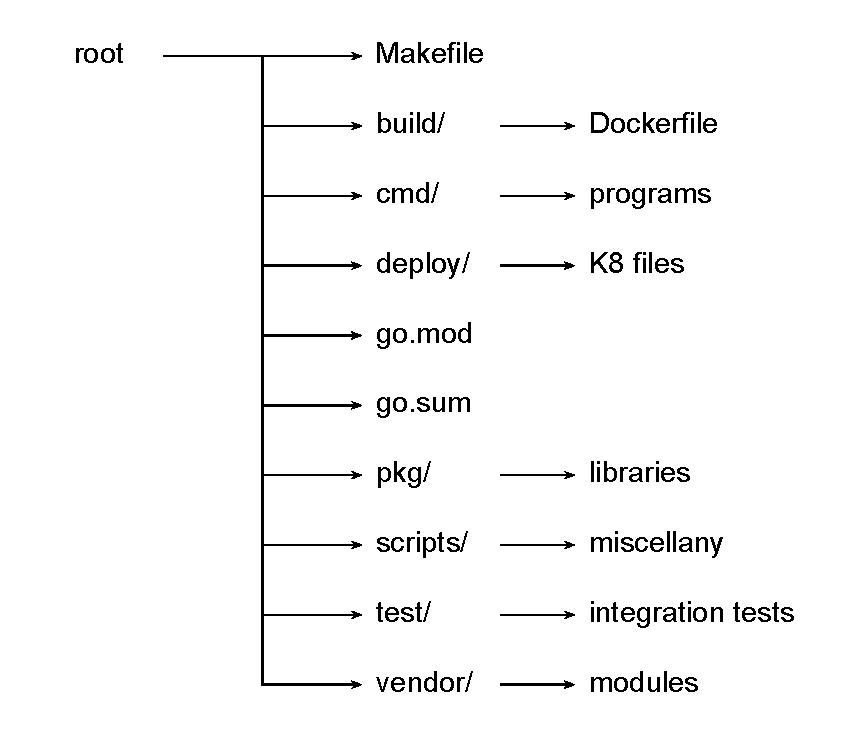
\includegraphics[height=.9\textheight]{dir-structure.pdf}
\end{center}
\end{frame}

\begin{frame}[fragile]
    \frametitle{Versioning the executable}
In the main program code:
\begin{golang}
// MUST BE SET by go build -ldflags "-X main.version=999"
// like 0.6.14-0-g26fe727 or 0.6.14-2-g9118702-dirty

// do not remove or modify
var version string
\end{golang}
See \href{https://medium.com/@joshroppo/setting-go-1-5-variables-at-compile-time-for-versioning-5b30a965d33e}%
{Setting compile-time variables for versioning} \par
\vspace{\baselineskip}
From the makefile:
{\scriptsize
\begin{verbatim}
version=$(shell git describe --tags --long --dirty 2>/dev/null)
branch=$(shell git rev-parse --abbrev-ref HEAD)

bvi: $(SOURCES)
    go build -mod=vendor -ldflags "-X main.version=$(version)" \
        -o $@ ./cmd/bvi
\end{verbatim}}
\end{frame}

\begin{frame}[fragile]
    \frametitle{Makefile extracts}
{\scriptsize
\begin{verbatim}
SOURCES := $(wildcard */*.go */*/*.go)

version=$(shell git describe --tags --long --dirty)

bvi: $(SOURCES)
	go build -mod=vendor -ldflags "-X main.version=$(version)" -o $@ ./cmd/bvi

bvi-linux: $(SOURCES)
	GOOS=linux GOARCH=amd64 CGO_ENABLED=0 go build -mod=vendor -a -tags netgo \
    -ldflags "-w" -ldflags "-X main.version=$(version)" -o $@ ./cmd/bvi

.PHONY: committed
committed:
	@git diff --exit-code >/dev/null || (echo "** NOT COMMITED **"; exit 1)

.PHONY: docker
docker: build/Dockerfile $(SOURCES)
	sed -e "/FIXME/s/FIXME/${version}/" -i.bak build/Dockerfile
	docker build -t sleigh-bvi:latest . -f build/Dockerfile
	mv build/Dockerfile.bak build/Dockerfile
\end{verbatim}}
\end{frame}

\begin{frame}[fragile]
    \frametitle{Building in Docker}
We can use Docker to build as well as run
\begin{itemize}
    \item Multi-stage builds
    \item Use a \verb|golang| image to build it
    \item Copy the results to a from-scratch image
\end{itemize}
\vspace{2\baselineskip}
The result is a small Docker container built for Linux \par
\vspace{\baselineskip}
And you can build it without even having Go installed! \par
\vspace{\baselineskip}
This is great for CI/CD environments
\end{frame}

\begin{frame}[fragile]
    \frametitle{Dockerfile extracts}
{\scriptsize
\begin{verbatim}
FROM golang:1.12.5-alpine3.9 AS builder
RUN /sbin/apk update && /sbin/apk --no-cache add ca-certificates git \
    tzdata && /usr/sbin/update-ca-certificates
RUN adduser -D -g '' bvi
WORKDIR /home/bvi
COPY go.mod /home/bvi
COPY go.sum /home/bvi
COPY vendor /home/bvi/vendor
COPY cmd    /home/bvi/cmd
COPY pkg    /home/bvi/pkg
RUN CGO_ENABLED=0 go build -mod=vendor -a -tags netgo -ldflags "-w" \
    -ldflags "-X main.version=FIXME" -o bvi ./cmd/bvi

FROM busybox:musl
COPY --from=builder /etc/ssl/certs/ca-certificates.crt /etc/ssl/certs/
COPY --from=builder /usr/share/zoneinfo /usr/share/zoneinfo
COPY --from=builder /etc/passwd /etc/passwd
COPY --from=builder /home/bvi/bvi /home/bvi
USER bvi
WORKDIR /home
EXPOSE 8444
ENTRYPOINT ["/home/bvi", "2>&1"]
\end{verbatim}}
\end{frame}

\begin{frame}[fragile]
    \frametitle{Discussion}
What questions do you have? \par
\vspace{0.4\baselineskip}
What else would you like me to talk about? \par
\vspace{1.6\baselineskip}
\begin{center}

\includegraphics[width=.6\textwidth]{grumpy-cat-90.jpg}
\par {\small\bf RIP Grumpy Cat 2012--2019}
\end{center}
\end{frame}


\end{document}
